\documentclass[]{article}
\usepackage[utf8]{inputenc}
\usepackage{hyperref}
\usepackage{graphicx}
\usepackage{color}

%opening
\title{Internship report}
\author{Aleksandr Samarin}
\date{2017}

\title{Internship report}
\begin{document}
\maketitle

\section{Introduction}
For 11 months from November 2014 till September 2015 I was working in TBricks AB, Swedish company that develops software technologies for trading on financial markets. I was assigned to the Quantitative Department (St. Petersburg's subdivision) as a Junior Software Engineer, where my major tasks were:
\begin{itemize}
	\item Implementation of different numerical methods (C/C++, Git)
	\item Maintenance of desktop applications that compute fair prices and greeks of European and American options according to tree models, Black-Scholes formulae and other mathematical models
	\item Development and implementation of curve-fitting algorithms
	\item Communication and negotiation with colleagues from different countries in English
	\item Business trips to Stockholm, Sweden
\end{itemize}

\section{Daily activities}
\subsection*{Implementation of curve-fitting algorithms} \
Most of the applications, developed by TBricks AB are based on financial mathematics. One of those applications was approximation of the data by specific curve. To clarify this task, let's first consider standard Black-Scholes formula for pricing of European call option:
\begin{equation}\label{bs}
	C(S, t) = S\Phi(d_1) - Ke^{-r(T-t)} \Phi(d_2),
\end{equation}
\[ d_1 = \frac{\ln(S / K) + (r + \sigma^2 / 2) (T - t) }{\sqrt{T-t}}, \]
\[ d_2 = d_1 - \sigma \sqrt{T-t}, \]
where
\begin{itemize}
	\item $C(S, t)$ -- current price of the option,
	\item $S$ -- current spot price of underlying asset,
	\item $\Phi(x)$ -- cumulative distribution function of standard normal distribution,
	\item $K$ -- strike price,
	\item $r$ -- risk-free rate,
	\item $T - t$ -- time to maturity,
	\item $\sigma$ -- volatility of underlying asset.
\end{itemize}

The aim is to get the so called \textbf{fair price} $C(S, t)$ -- the value to which traders will refer in order to price the option. The problem is that all the parameters are known and well-defined except volatility $\sigma$. How should we estimate it? \\

One of the possible ways is \textbf{implied volatility}. Firstly, we get option bid-ask prices from the market and insert them into the equation \ref{bs}. Then we obtain corresponding implied volatilities via Newton root-finding procedure. \\

My personal task was to determine parameters of specific curve in a way it fits implied volatilities the best.
The desired properties of the curve would be its sufficient smoothness and passage through bid-ask spread for each strike, especially near At-The-Money point. However, due to specificity of the curve it's not always possible. \\
\begin{figure}
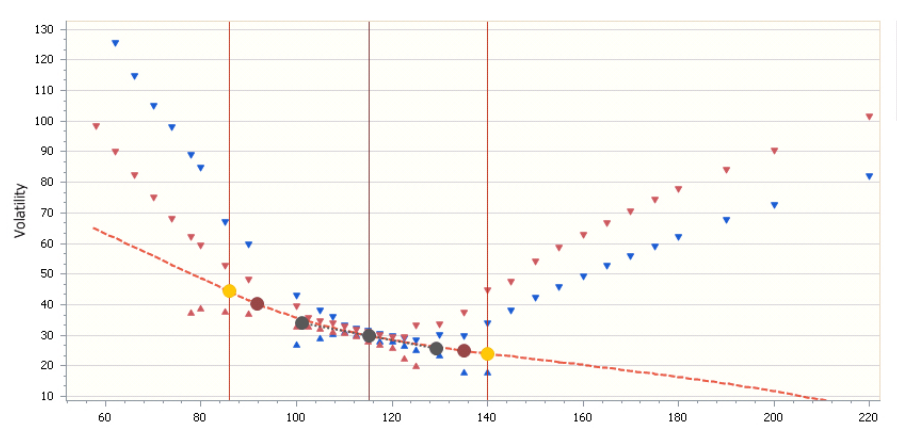
\includegraphics[scale=0.5]{iv}
\caption{Screenshot from the real software environment. Dependency of volatility from strike. {\color{red}Red} triangles correspond to call options, {\color{blue}blue}  -- to put options. If triangle looks up -- this is bid, otherwise -- this is ask. On the picture one can see well-known phenomena -- \textbf{volatility smile} (different strikes imply different volatilities).}
\end{figure}
\
The sought-for curve is an attempt to describe the volatility behavior. I was considering following models of volatility curves:
\begin{itemize}
	\item Parabola with different curvature and slope parameters for call/put options -- the way to imitate volatility smile,
	\item Weighted cubic splines -- perfect tool for regression
\end{itemize}
The objective function that we want to minimize is
\[
\sum_i (f(K_i) - \sigma_i)^2,
\]
where $f$ -- function of the curve,  $K_i$ -- strike price and $\sigma_i$ -- implied volatility.
Perfect curve shouldn't be just found, but it also should be found as fast as possible. In the case of parabola there was used Levenberg-Marquardt algorithm to solve constrained optimization problem. In the case of cubic splines I was using algorithm, described in the book of Paul Dierckx ``Curve and Surface fitting with splines'' \\

Then the aforementioned fair-price is calculated again from the equation \ref{bs}, where $\sigma$ is taken from the curve.

\subsection*{Pricing models support} \
In order to calculate price of the options, quantitative department of TBricks AB has implemented three different methods:
\begin{itemize}
	\item Crank-Nicolson finite-difference scheme,
	\item Binomial tree model
	\item Trinomial tree model
\end{itemize}
Finite-difference scheme provides better accuracy, however, this method is too slow to use in the real market conditions. That's why most of the clients of TBricks AB have preferred to use binomial tree model.
My part was the integration of trinomial tree model, which works in the similar way as binomial, except that amount of branches has been increased to three. This improvement has allowed to add one more degree of freedom to the tree model equations. Consequently, trinomial model has speed of convergence comparative with finite-difference scheme and works as fast as binomial one. More details can be found in Master thesis of Walter Nordström ``Adaptive tree techniques in option pricing''.
\begin{figure}
	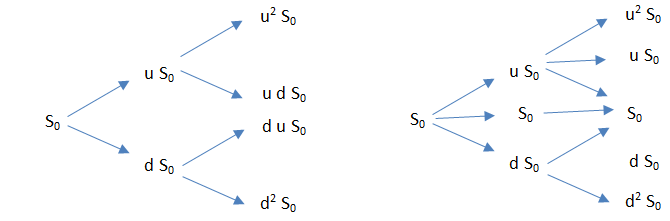
\includegraphics[scale=0.5]{bm}
	\caption{Comparison of binomial and trinomial tree pricing models.}
\end{figure}

\subsection*{Working with international colleagues across time-zones} \
My personal duties were not limited solely by developing mathematical models, but also included interaction with colleagues from different countries. I received e-mails and calls through Skype from different offices of Support Department, located in Stockholm, London, Chicago and Hong Kong. I was responsible for explanation of subtle work details of various models. If it was necessary, I needed to change them. One of the examples was an argue between Raiffeisen Bank and City Bank, that couldn't agree on how to price bonds. During bond's lifetime there were paid coupons and price of the bond was dropping respectively to the value of the coupon on the same day. Traders from Raiffeisen Bank wanted price of the bond to be dropped before the day of paying coupon, however City Bank wanted to have price dropping the day after. In the first case price of the bond would be dropping the day before maturity and that would affect City Bank strongly. Meanwhile, Raiffeisen traders weren't pricing bonds, whose time to maturity was less than a week, as they were considering only coupons. I decided to solve the problem in the following way: price of the bond will drop the day before coupon date, but only if it's not the day of maturity. Otherwise, the price will drop after. This trade-off has allowed both banks to use the same application without any inconvenience for themselves.

Furthermore, there were not only calls, but also business trips from St. Petersburg to Stockholm, during which I had negotiations with colleagues from quantitative department and was learning new mathematical models in finance.

\section{Summary}
\
Overall, I had a great practical experience in financial mathematics.
I've learned a lot of new ideas through books and conversations with co-workers, could apply them in practice and see the result instantly.
I've learned the nuances of daily work of quantitative engineer and I'm very grateful to TBricks AB for this opportunity.

\section{Useful literature}
\begin{enumerate}
	\item Paul Dierckx ``Curve and Surface fitting with splines''
	\item Walter Nordström ``Adaptive tree techniques in option pricing''
\end{enumerate}

\end{document}
